\section{Clustering}
\emph{Most of the figures presented in this section are also available in 
appendix~\ref{app:larger-figures} as larger versions.}

\subsection{Small Data Set Activity Detection}
This section addresses data sets consisting of $822$ Moments, ranging 
from a few data points to thousands in each set. All three algorithms
have been given an attempt to cluster each Moment. The
\emph{haversine}\footnote{
    The haversine function, also called the great circle distance, 
    takes the curvature of the earth in consideration when measuring long
    distances between latitudes and longitudes \cite{haversine}.
} method is used for distance measurements. A computation is aborted if 
it takes longer than $100$ seconds, as the clustering is intended to be 
done automatically and in real-time\footnote{
    This is implied by the server-side placement of the clustering algorithm, and the intention to automate the process. For an automated service in the
    cloud with many users, the cost of CPU computations are not feasible
    if a service such as this takes more than a few seconds. 
}, where a run-time of close to a minute is not feasible. Results are 
excluded from a algorithms computation result set if it did not finish 
in time. In total, CLARANS timed out on $43$ of the Moments, and 
DBSCAN and SLINK did the same with $1$ each.

\subsubsection{Performance}

\begin{figure}[ht!]
    \centering
    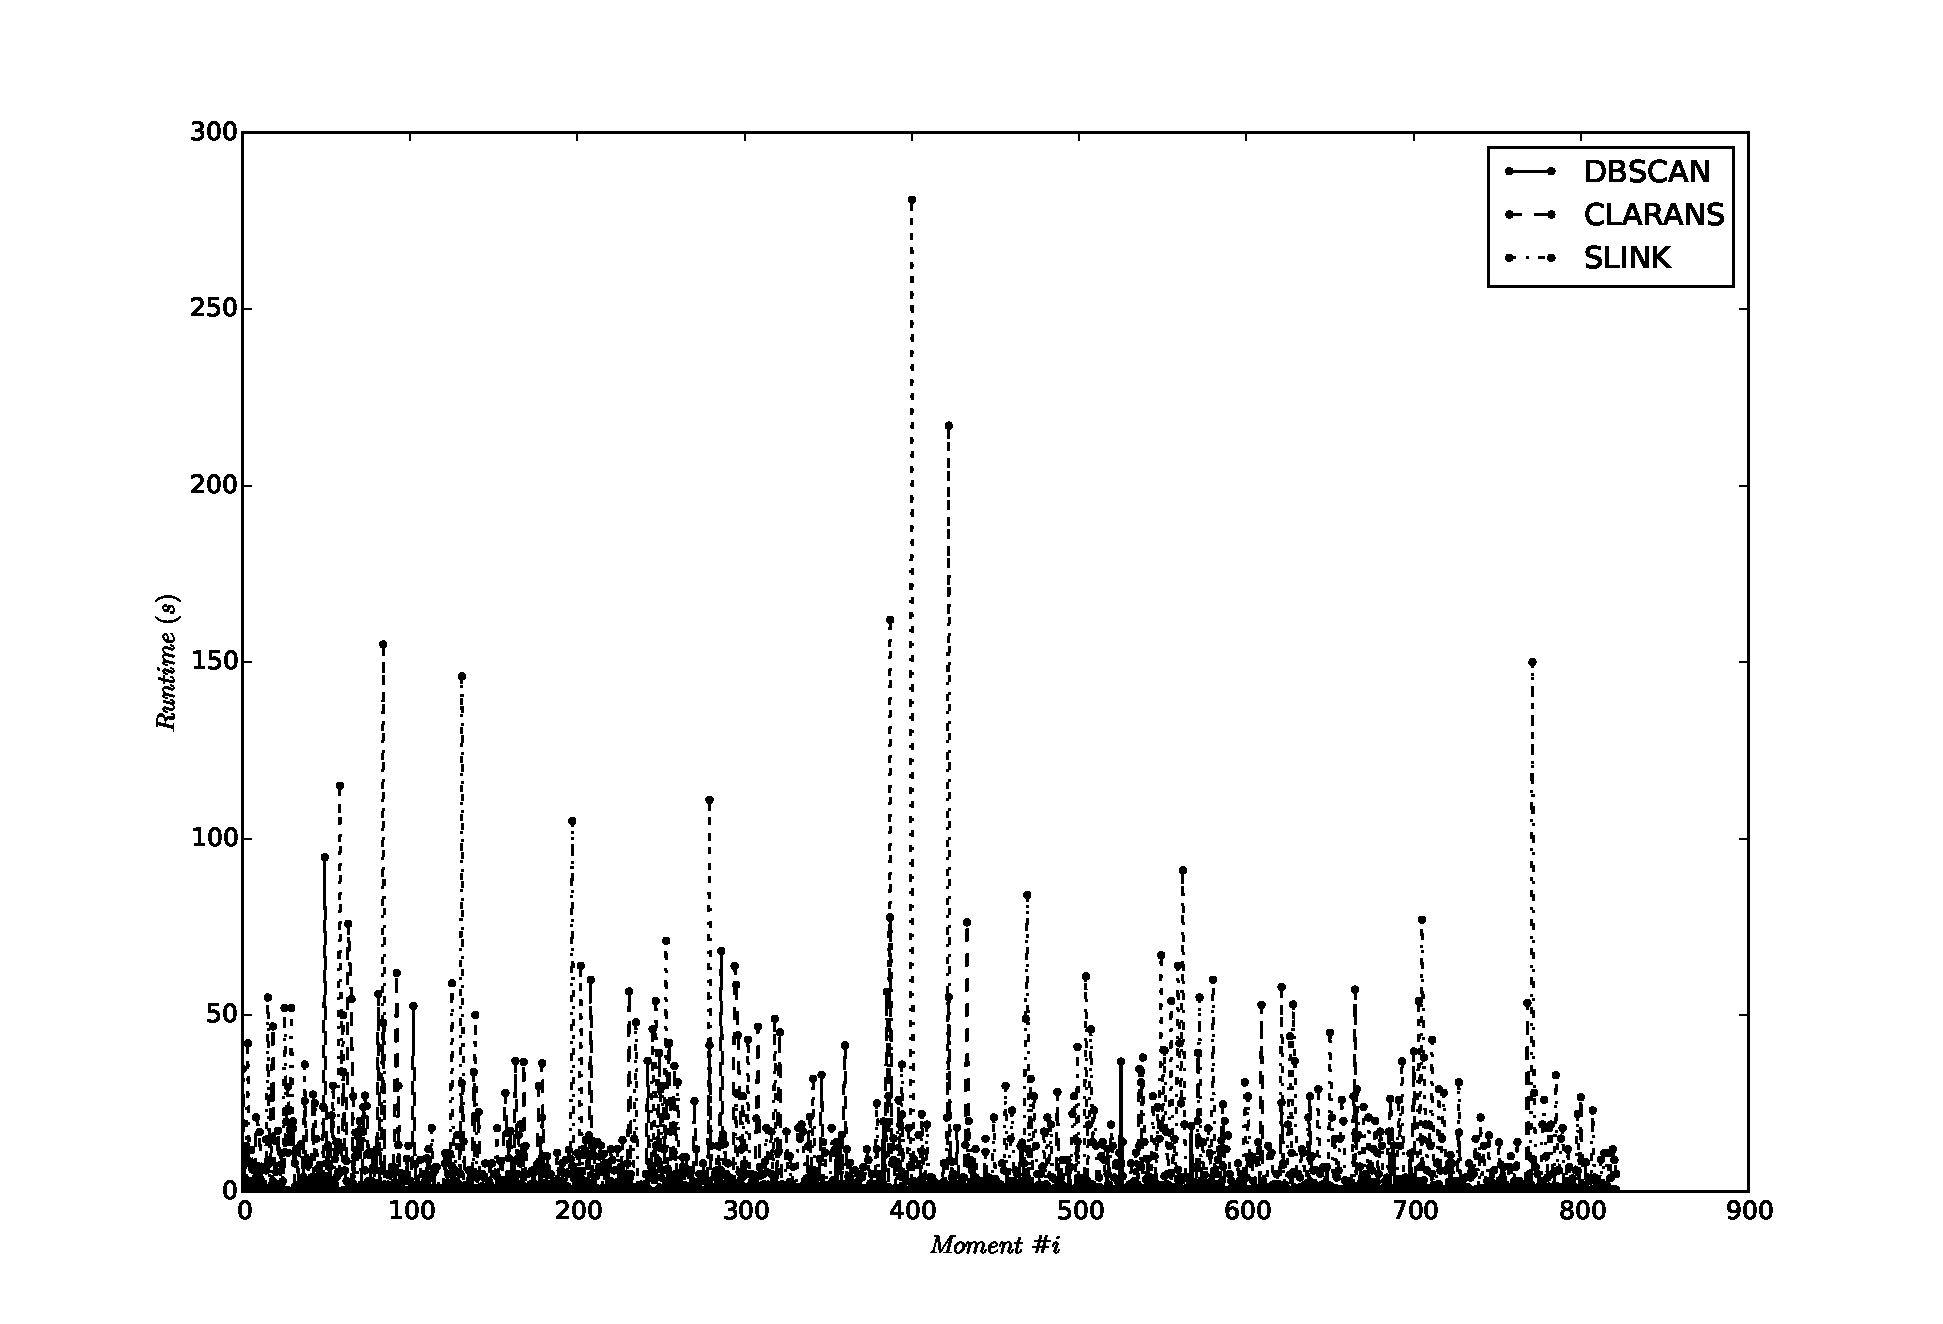
\includegraphics[width=0.9\textwidth]{plots/moment_runtime_plot.pdf}
    \caption{Run-time for clustering algorithms over Moments.
    \label{fig:moment-runtime-plot} }
\end{figure}

%%%%%%%%%%%%%%%%%%%%%%%%%%%%%%%%%%%%%%%%%%%% 80 line marker %%%%%%%%%%%%%%%
To evaluate the efficiency of the algorithms, the run-time for 
each algorithm over various Moments is plotted. 
Figure~\ref{fig:moment-runtime-plot} provides an overview over the run-time 
on Moments ordered randomly\footnote{
    The Moments in this plot is actually ordered by an internal Moment ID 
    provided by the database, although this is not of importance in this 
    section. For all intents and purposes, these are randomly ordered.
}. 
 
\begin{figure}[ht]
    \centering
    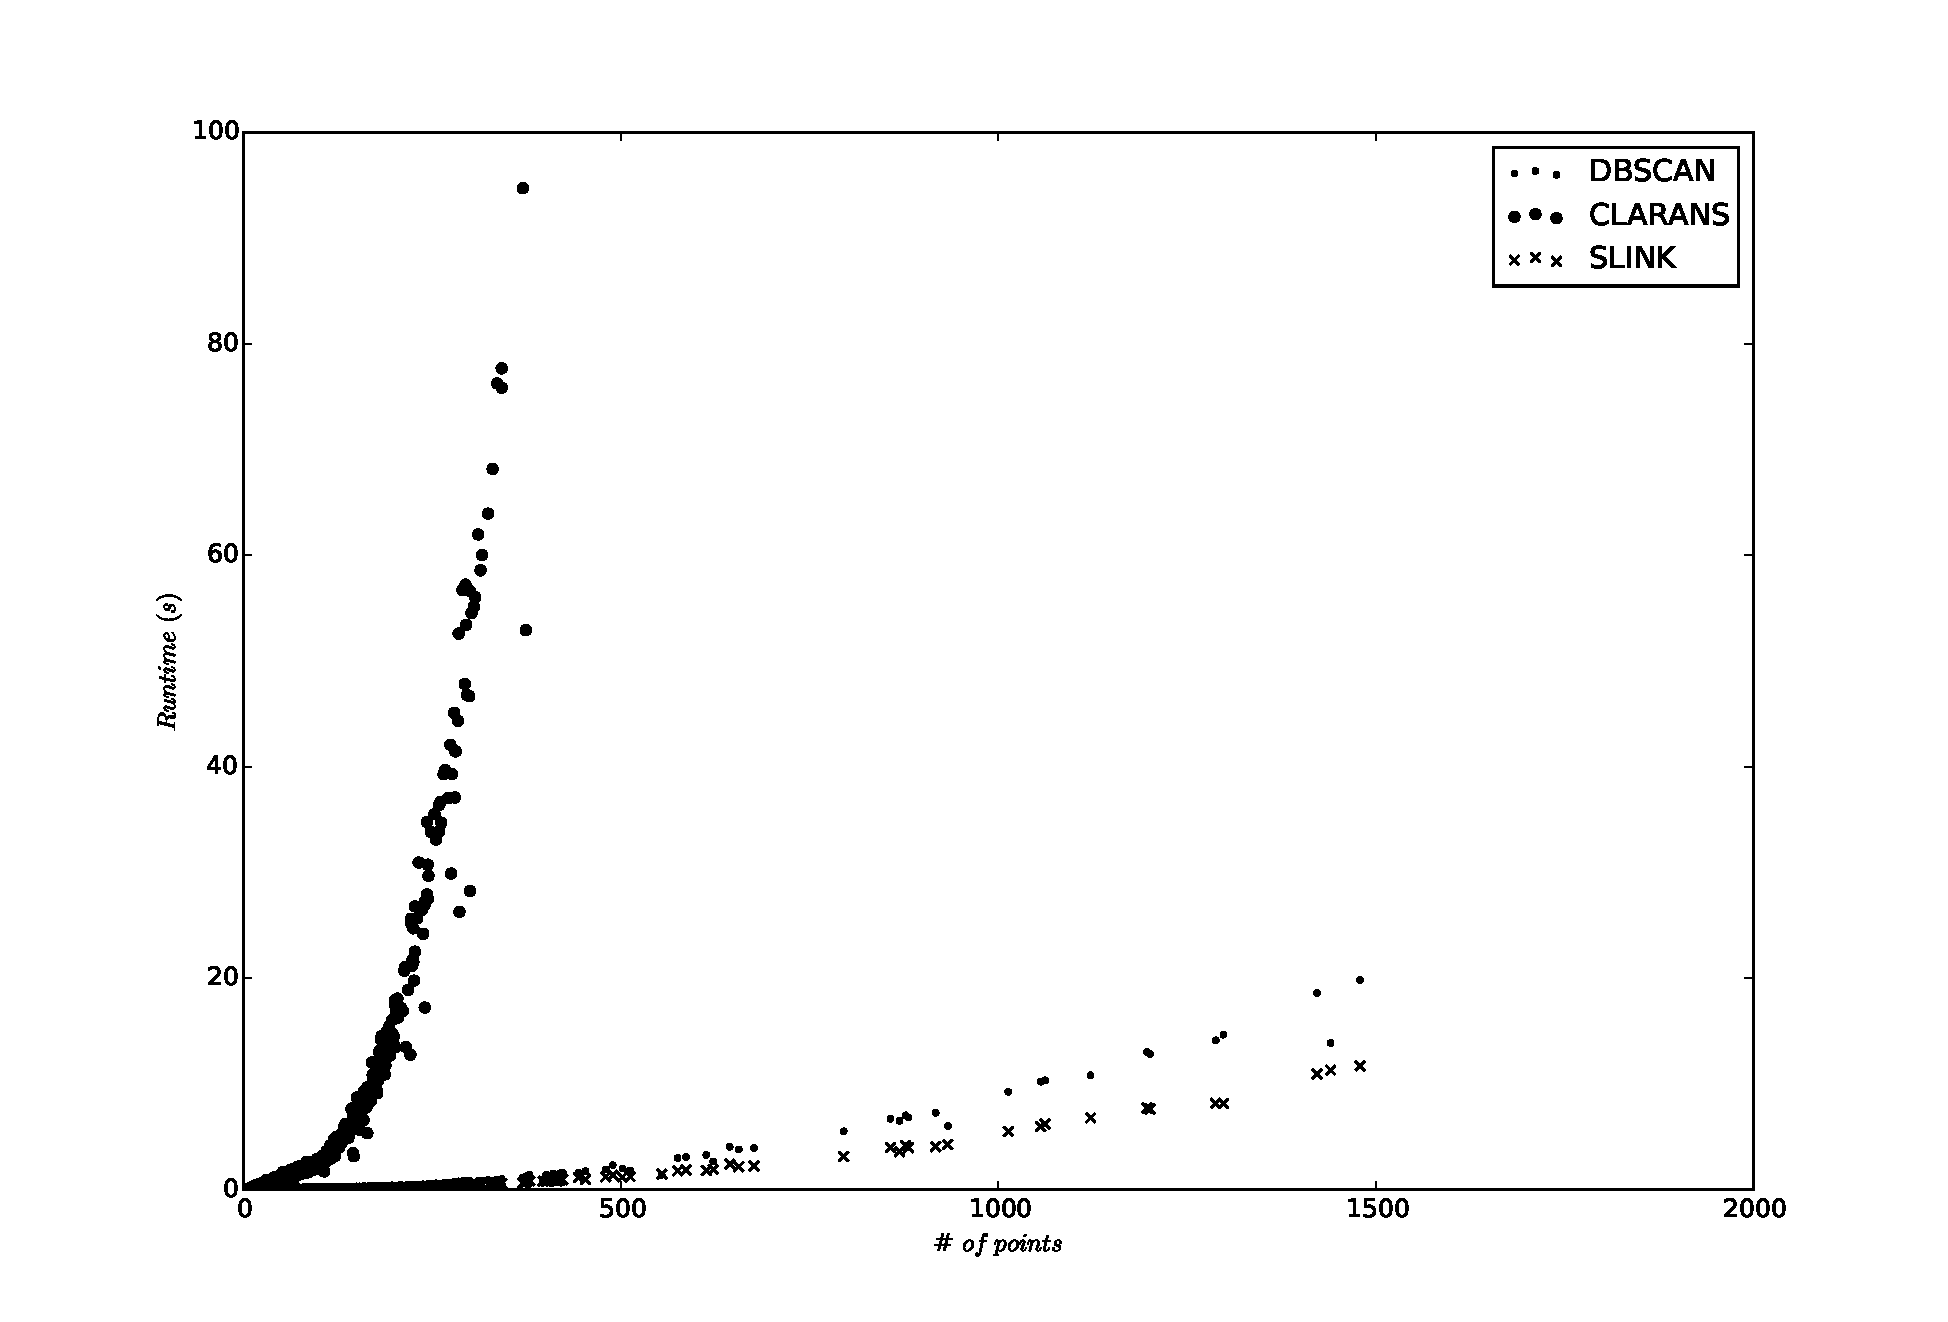
\includegraphics[width=0.9\textwidth]{plots/moment_runtime_scatter.pdf}
    \caption{Run-time for clustering algorithms over Moments, by number of
        points in the Moment.
    \label{fig:moment-runtime-scatter} }
\end{figure}

A more intuitive view is provided by figure~\ref{fig:moment-runtime-scatter}, 
where the run time of each point is mapped with the number of points in each 
Moment. This obviously provides a hint towards the time-complexity of each 
algorithm, which becomes quite clear. 

\cleartoleftpage

\subsubsection{Silhouettes}

\begin{figure}[ht]
    \centering
    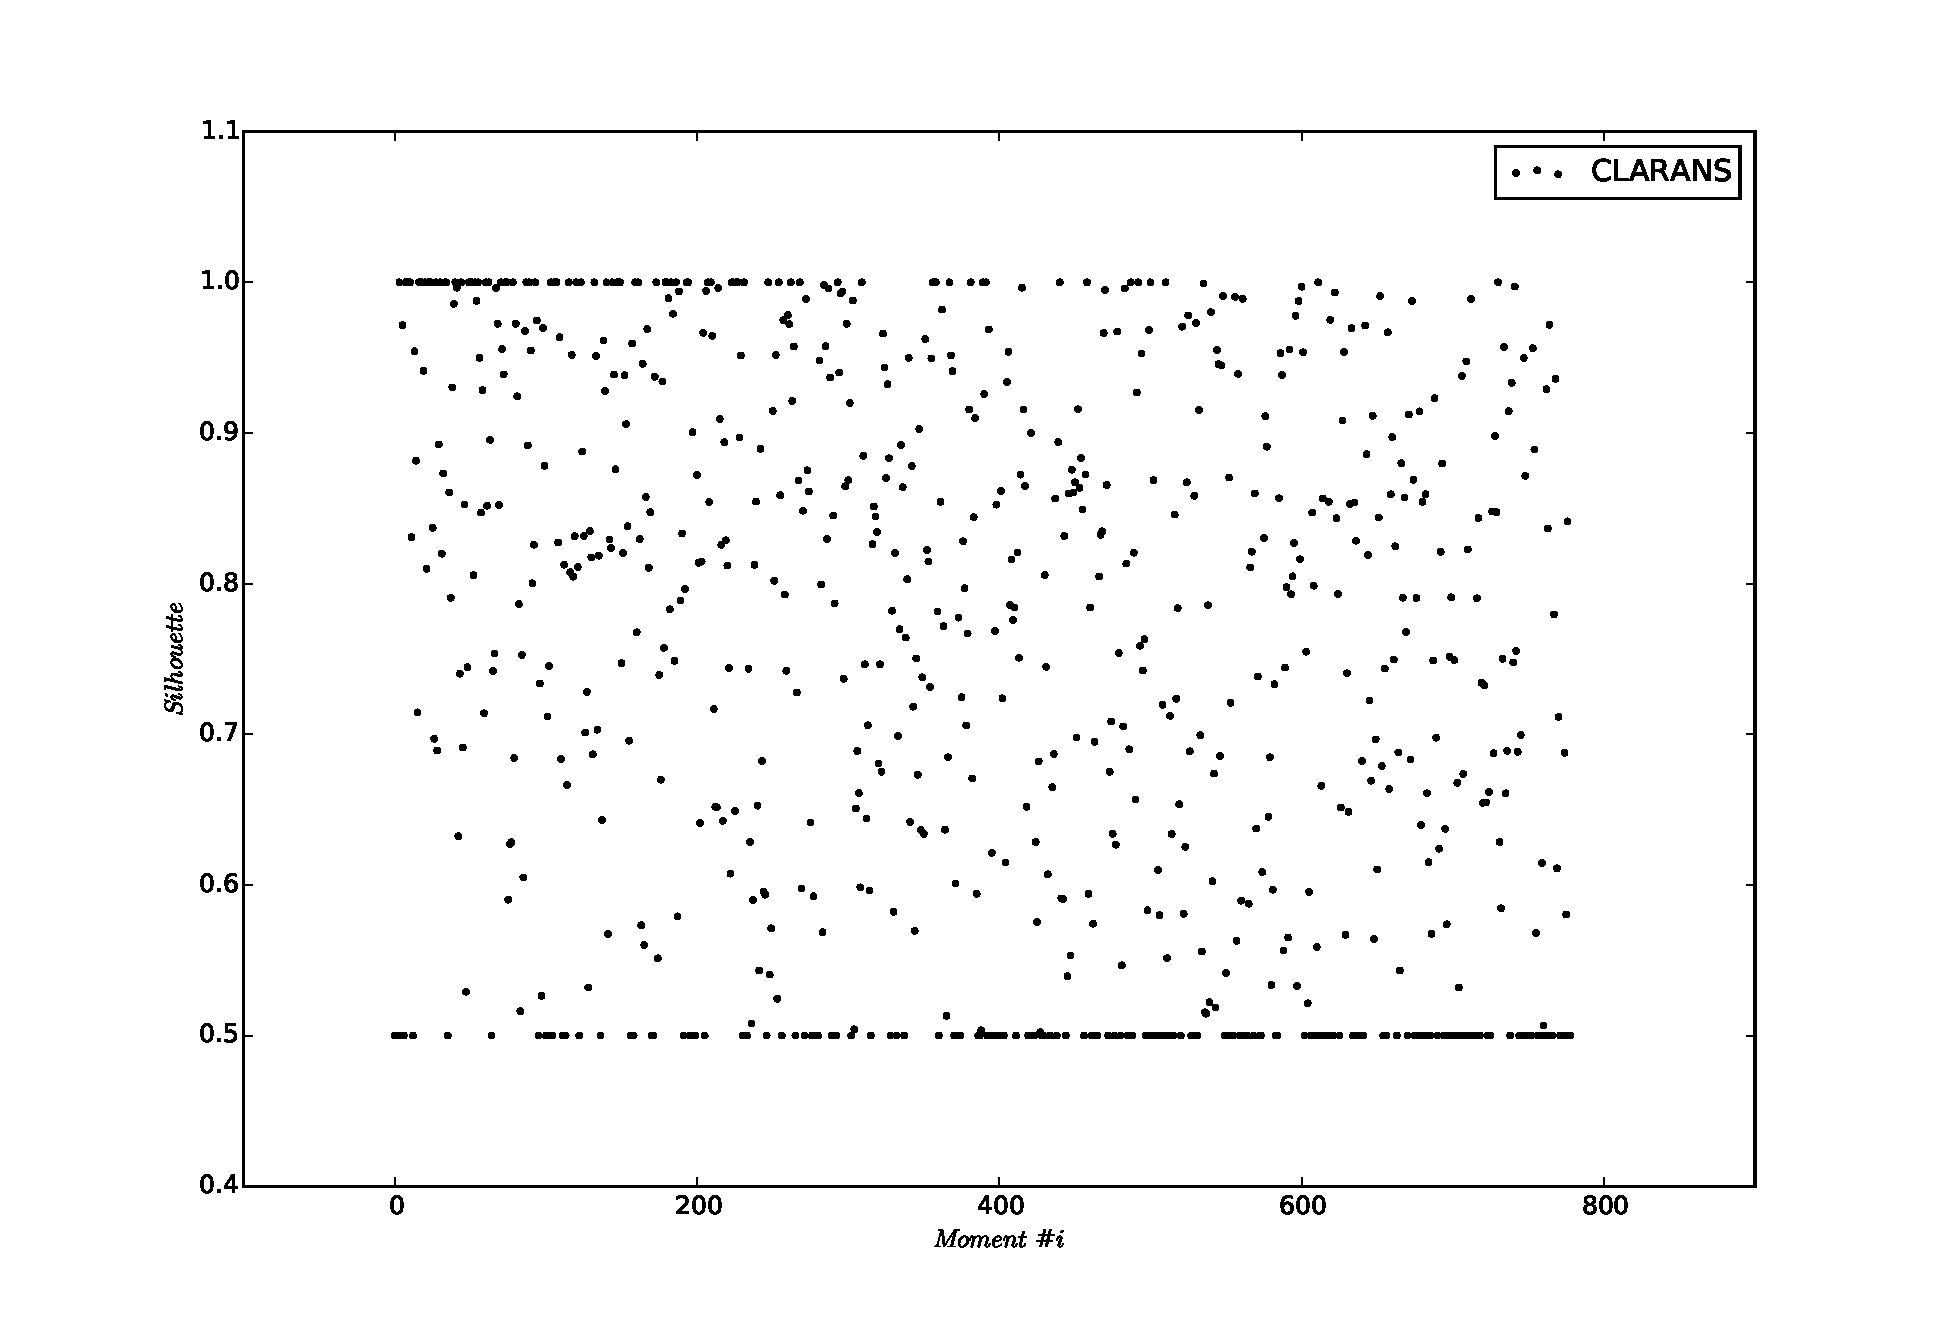
\includegraphics[width=0.9\textwidth]{plots/clarans_silhouette.pdf}
    \caption{Moment-wise silhouette coefficients for CLARANS.
    \label{fig:clarans-silhouette} }
\end{figure}

\begin{figure}[ht]
    \centering
    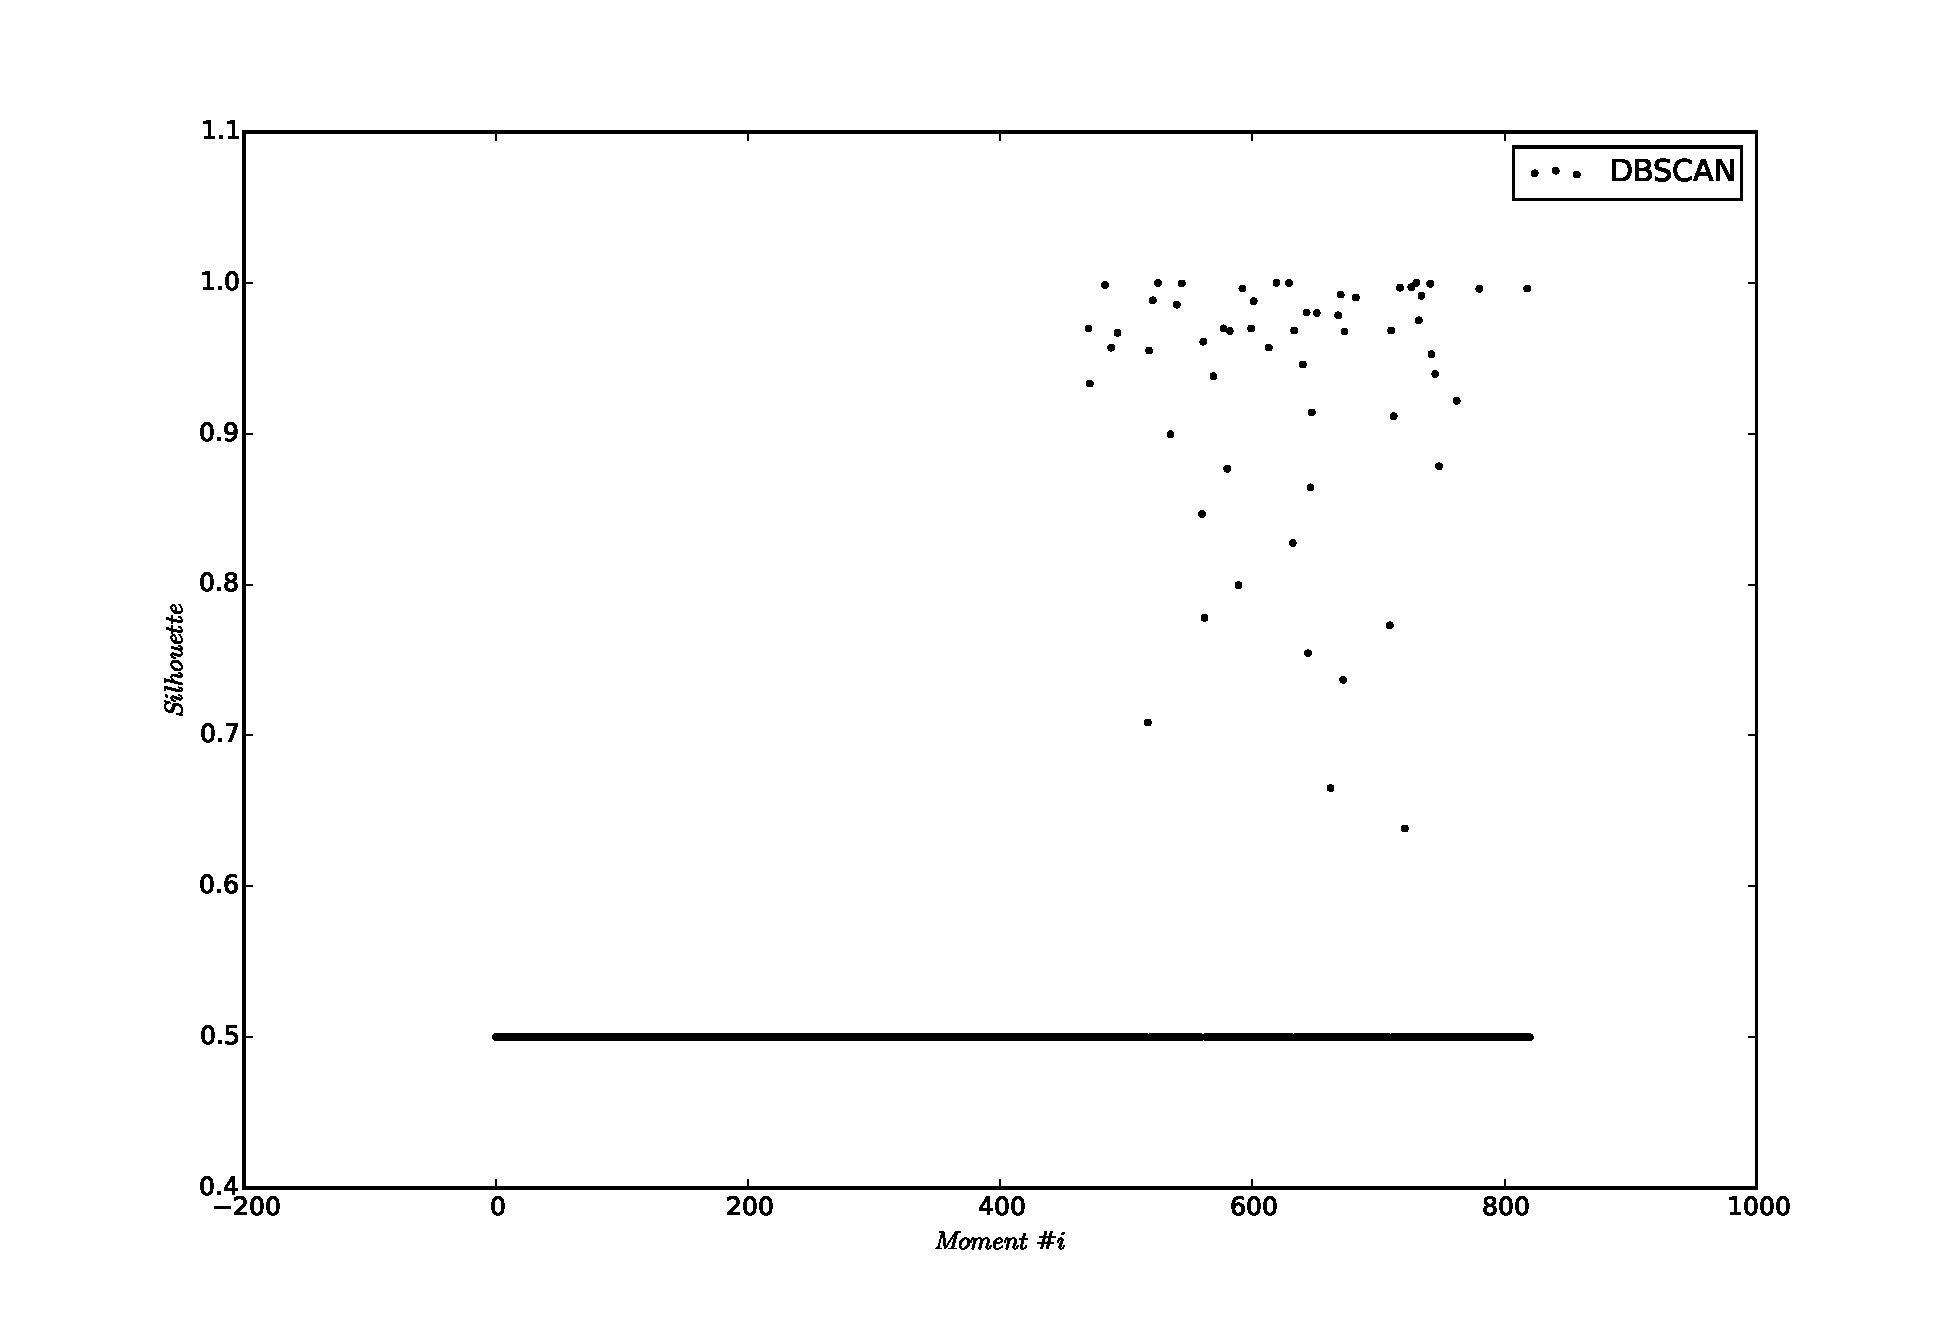
\includegraphics[width=0.9\textwidth]{plots/dbscan_silhouette.pdf}
    \caption{Moment-wise silhouette coefficients for DBSCAN.
    \label{fig:dbscan-silhouette} }
\end{figure}

\begin{figure}[ht]
    \centering
    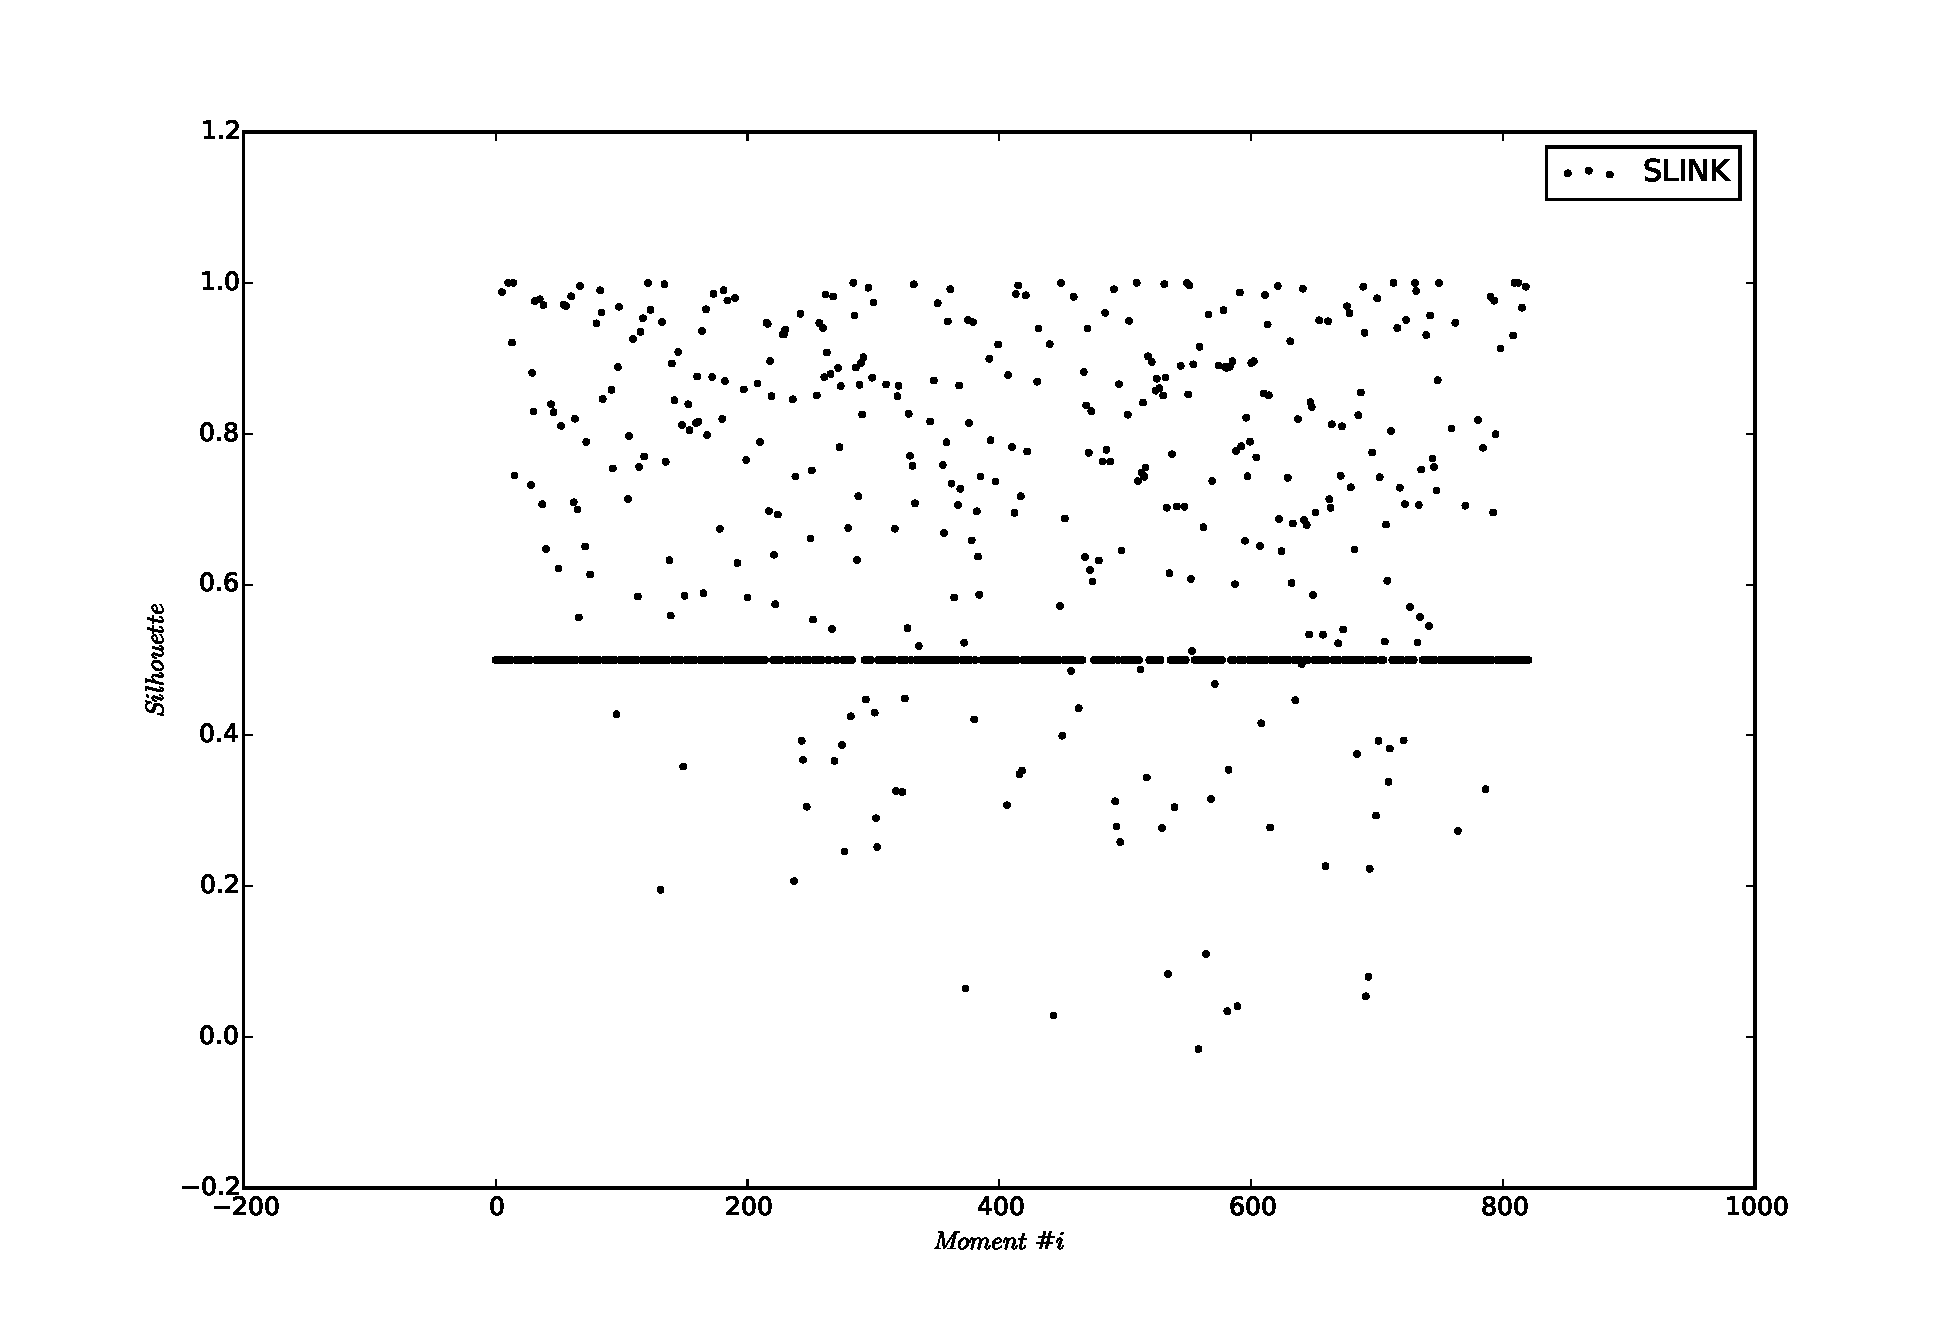
\includegraphics[width=0.9\textwidth]{plots/slink_silhouette.pdf}
    \caption{Moment-wise silhouette coefficients for SLINK.
    \label{fig:slink-silhouette} }
\end{figure}

\begin{table}
    \centering
    {\begin{tabular}{ | l | l | c c c c | }
        \hline
        Algorithm & Mean SC        & Strong & Reasonable & Weak & No  \\
        \hline
        CLARANS   & 0.751818981799 & 457    & 167        & 155  & 0  \\
        DBSCAN    & 0.529126434287 & 54     & 2          & 765  & 0  \\
        SLINK     & 0.608986935167 & 250    & 69         & 486  & 16 \\
        \hline
    \end{tabular}}
    \caption{Mean silhouette coefficient per algorithm in the data set, and
        quantities within each defined Silhouette interpretation area.} 
    \label{table:mean-silhouette}
\end{table}

The Silhouette coefficients are plotted with the Moments sorted from 
the smallest number of data points to the largest, shown in 
figure~\ref{fig:clarans-silhouette}, figure~\ref{fig:dbscan-silhouette}
and figure~\ref{fig:slink-silhouette}. The sorting is intended
to visualize any potential correlation between the number of data points 
in a set, and the clustering results with regard to Silhouette coefficients.

The mean value of each plot is provided as a more comprehensible reference 
value in table~\ref{table:mean-silhouette}, along with the quantities of
coefficients with in each interpretation category, 
as suggested by \citeauthor{silhouettes}.

\cleartoleftpage

\subsection{Larger Data Set Activity Detection}
This section addresses data set consisting of $59$ photo sequences
grouped by user id's, ranging 
from $200$ data points to thousands in each set. All three algorithms
have been given an attempt to cluster each photo sequence. The \emph{haversine} 
method is used for distance measurements. A computation is aborted if 
it takes longer than $60$ seconds. Results are 
excluded from a algorithms computation result set if it did not finish
in time. In total, CLARANS timed out on $19$ of the Moments, and 
DBSCAN and SLINK did the same with $1$ each. In this data sets, multiple
clusters are likely to be present, as it contains several Moments in 
each data set. 

\subsubsection{Performance}

\begin{figure}[ht]
    \centering
    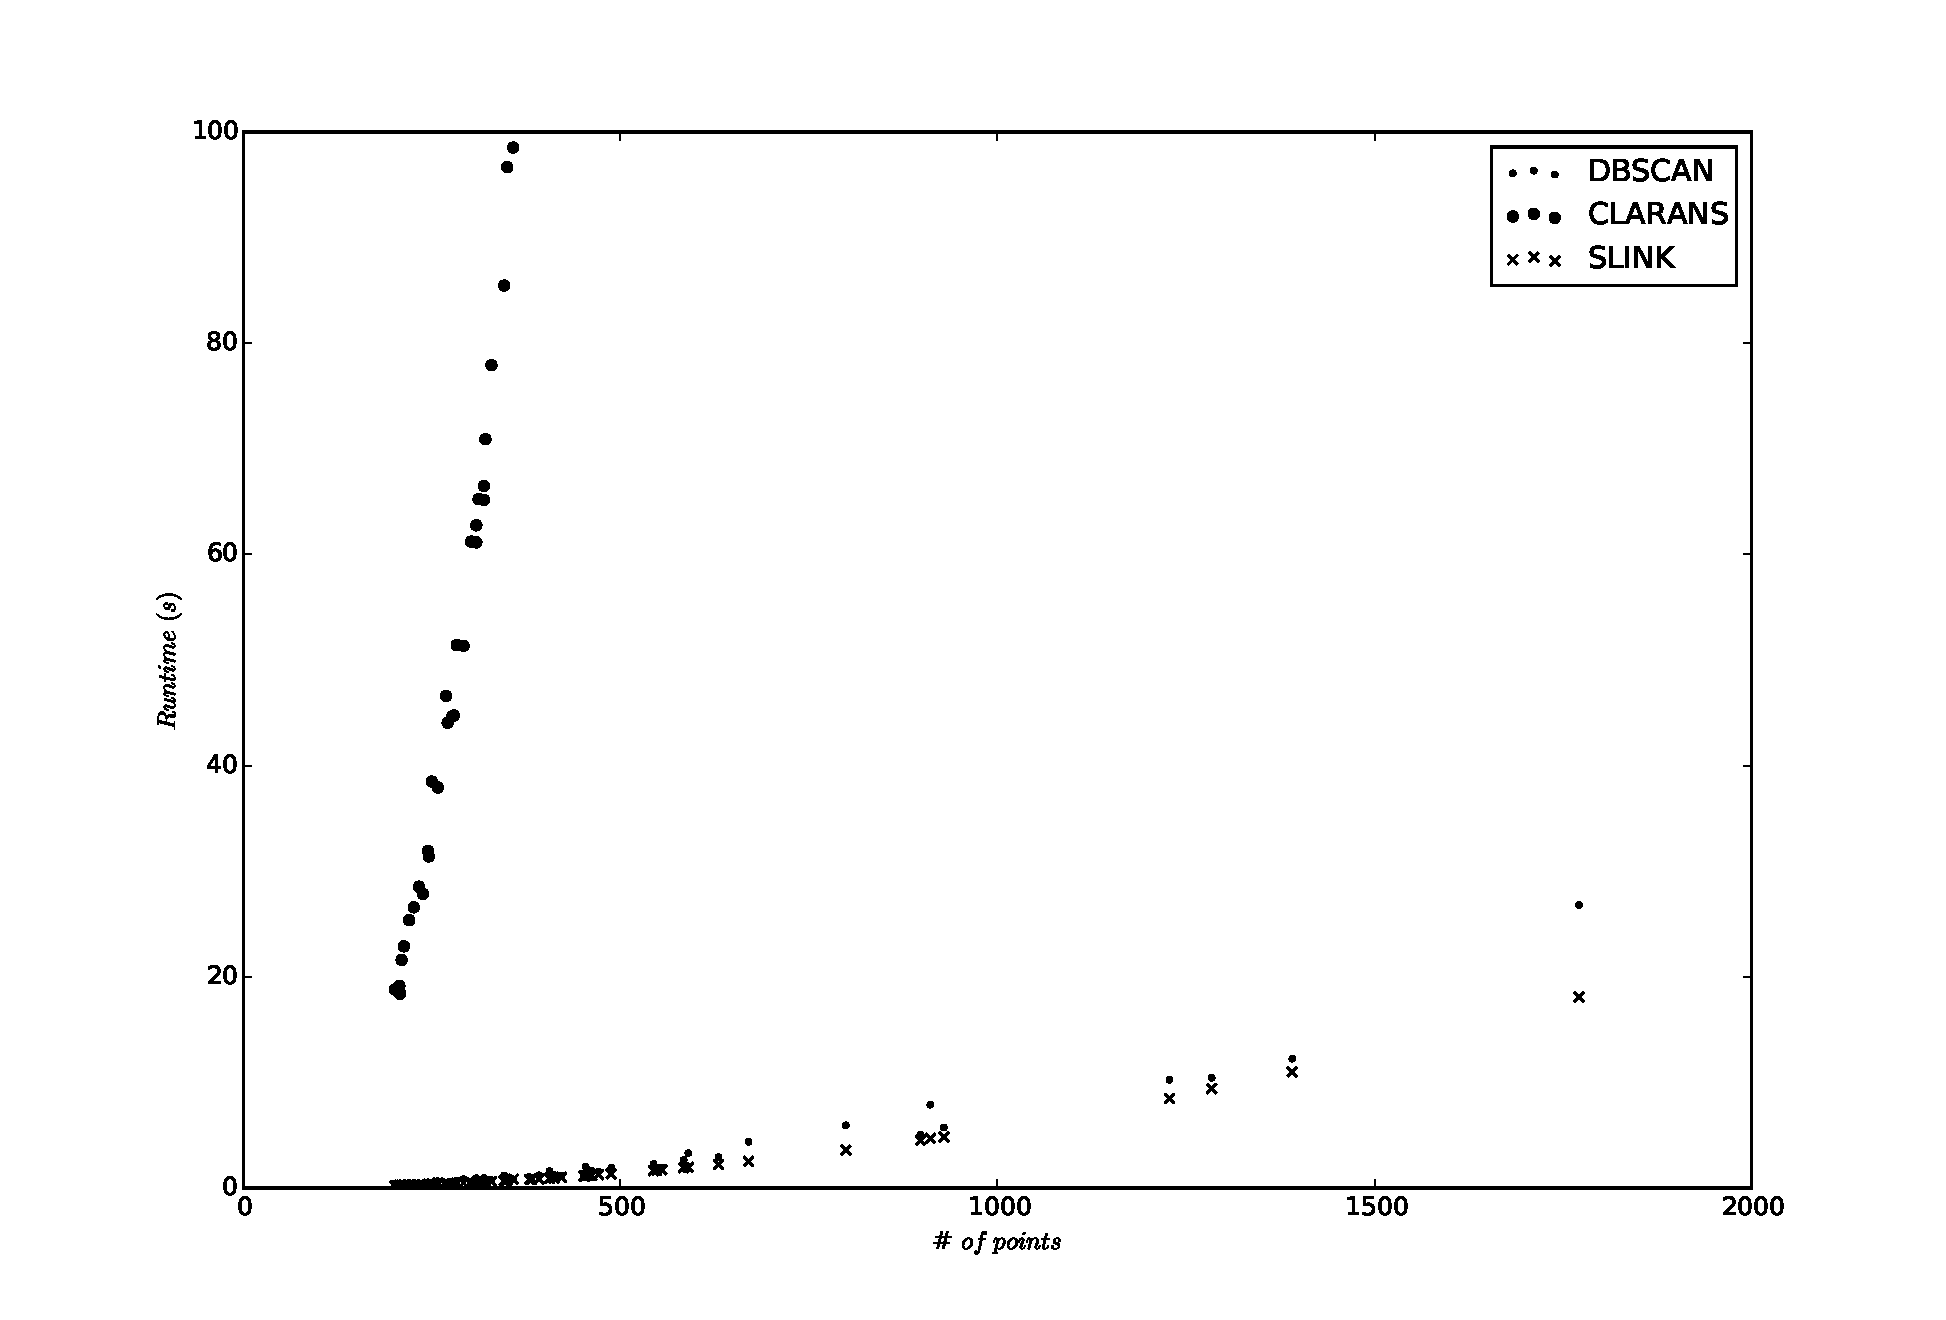
\includegraphics[width=0.7\textwidth]{plots/days_runtime_scatter.pdf}
    \caption{Run-time for clustering algorithms over users days, by number of
        points on the day.
    \label{fig:day-runtime-scatter} }
\end{figure}

The plot depicting run-time in figure~\ref{fig:day-runtime-scatter} now 
shows somewhat smaller spectrum of the x-axis.

\clearpage

\subsubsection{Silhouettes}

The Silhouettes have not changed from the smaller data set in any particular
manner, and are therefore shown here for completeness.

\begin{table}
    \centering
    {\begin{tabular}{ | l | l | c c c c | }
        \hline
        Algorithm & Mean SC & Strong & Reasonable & Weak & No  \\
        \hline
        CLARANS & 0.783864065615 & 19 & 9 & 2  & 0  \\
        DBSCAN  & 0.581829108024 & 10 & 0 & 48 & 0  \\
        SLINK   & 0.63724366955  & 20 & 6 & 32 & 0  \\
        \hline
    \end{tabular}}
    \caption{Mean silhouette coefficient per algorithm in the larger data set, and
        quantities within each defined Silhouette interpretation area.} 
    \label{table:days-mean-silhouette}
\end{table}

\begin{figure}[h!]
    \centering
    \begin{subfigure}[b]{0.45\textwidth}
        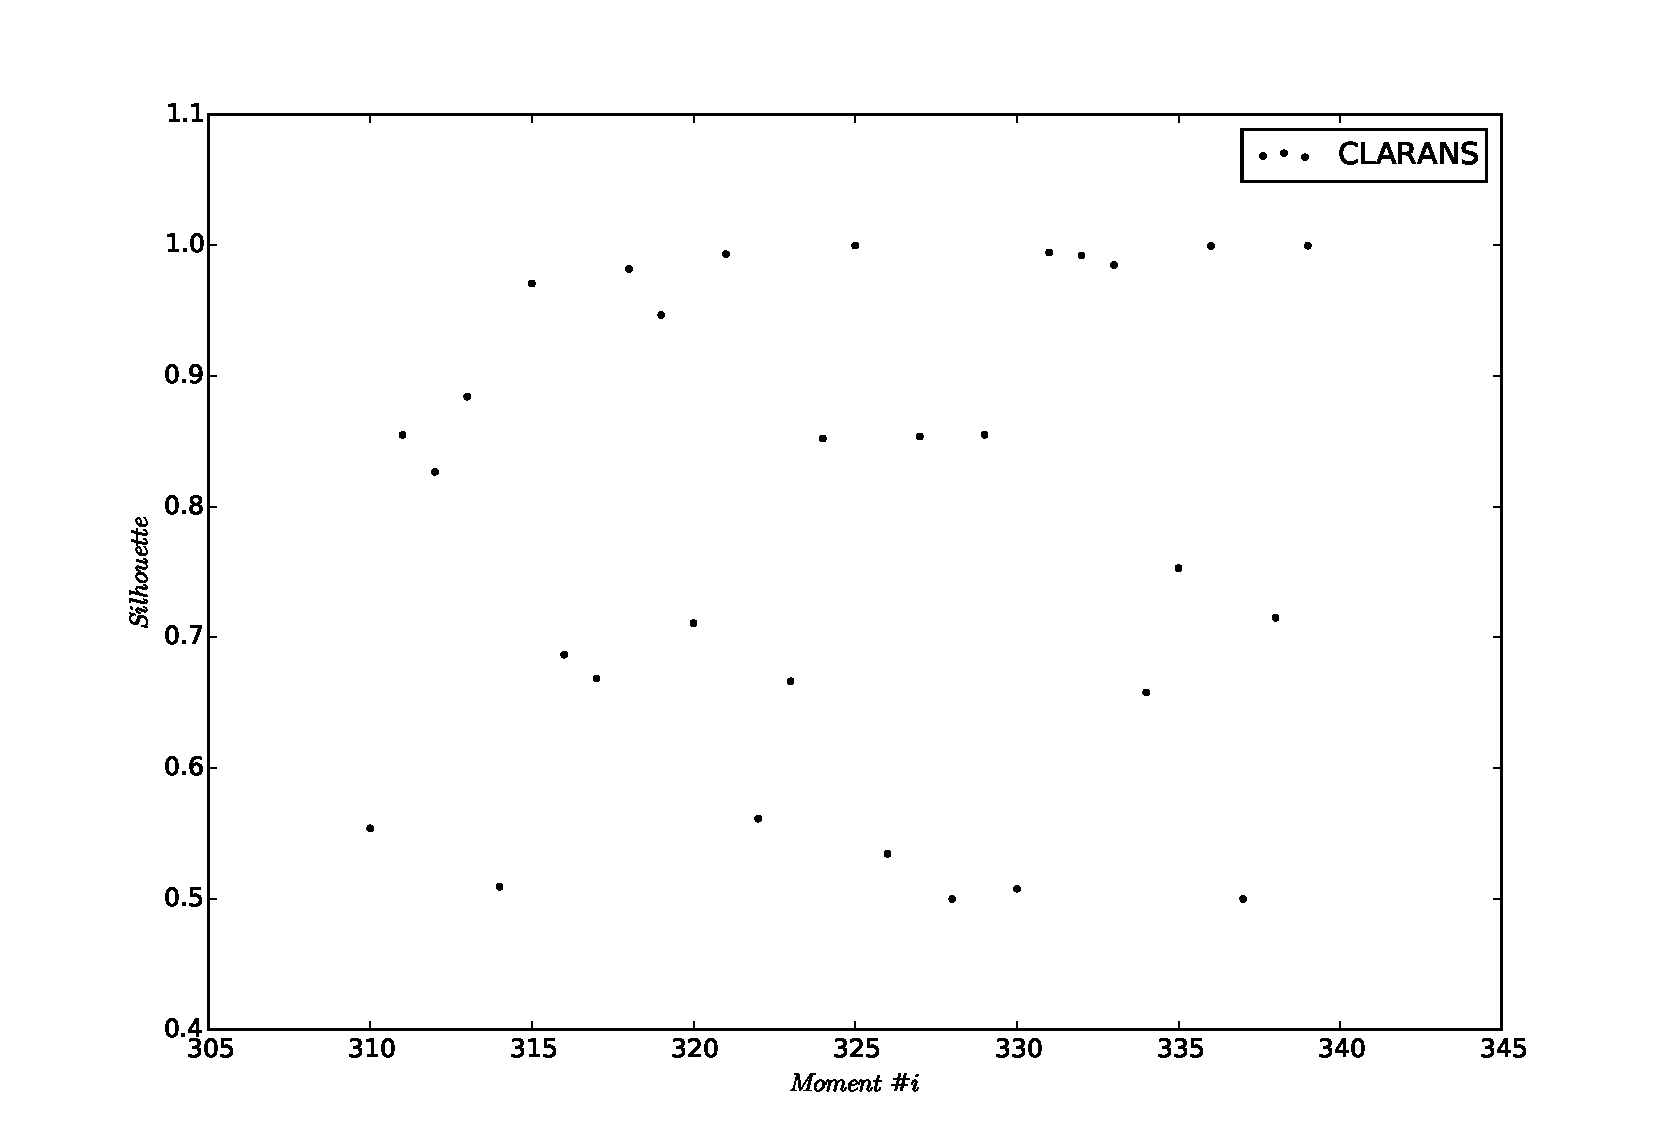
\includegraphics[width=\textwidth]{plots/days_clarans_silhouette.pdf}
        \caption{Moment-wise silhouette coefficients for CLARANS for a larger 
        data set. }
        \label{fig:days-clarans-silhouette}
    \end{subfigure}%
    ~
    \begin{subfigure}[b]{0.45\textwidth}
        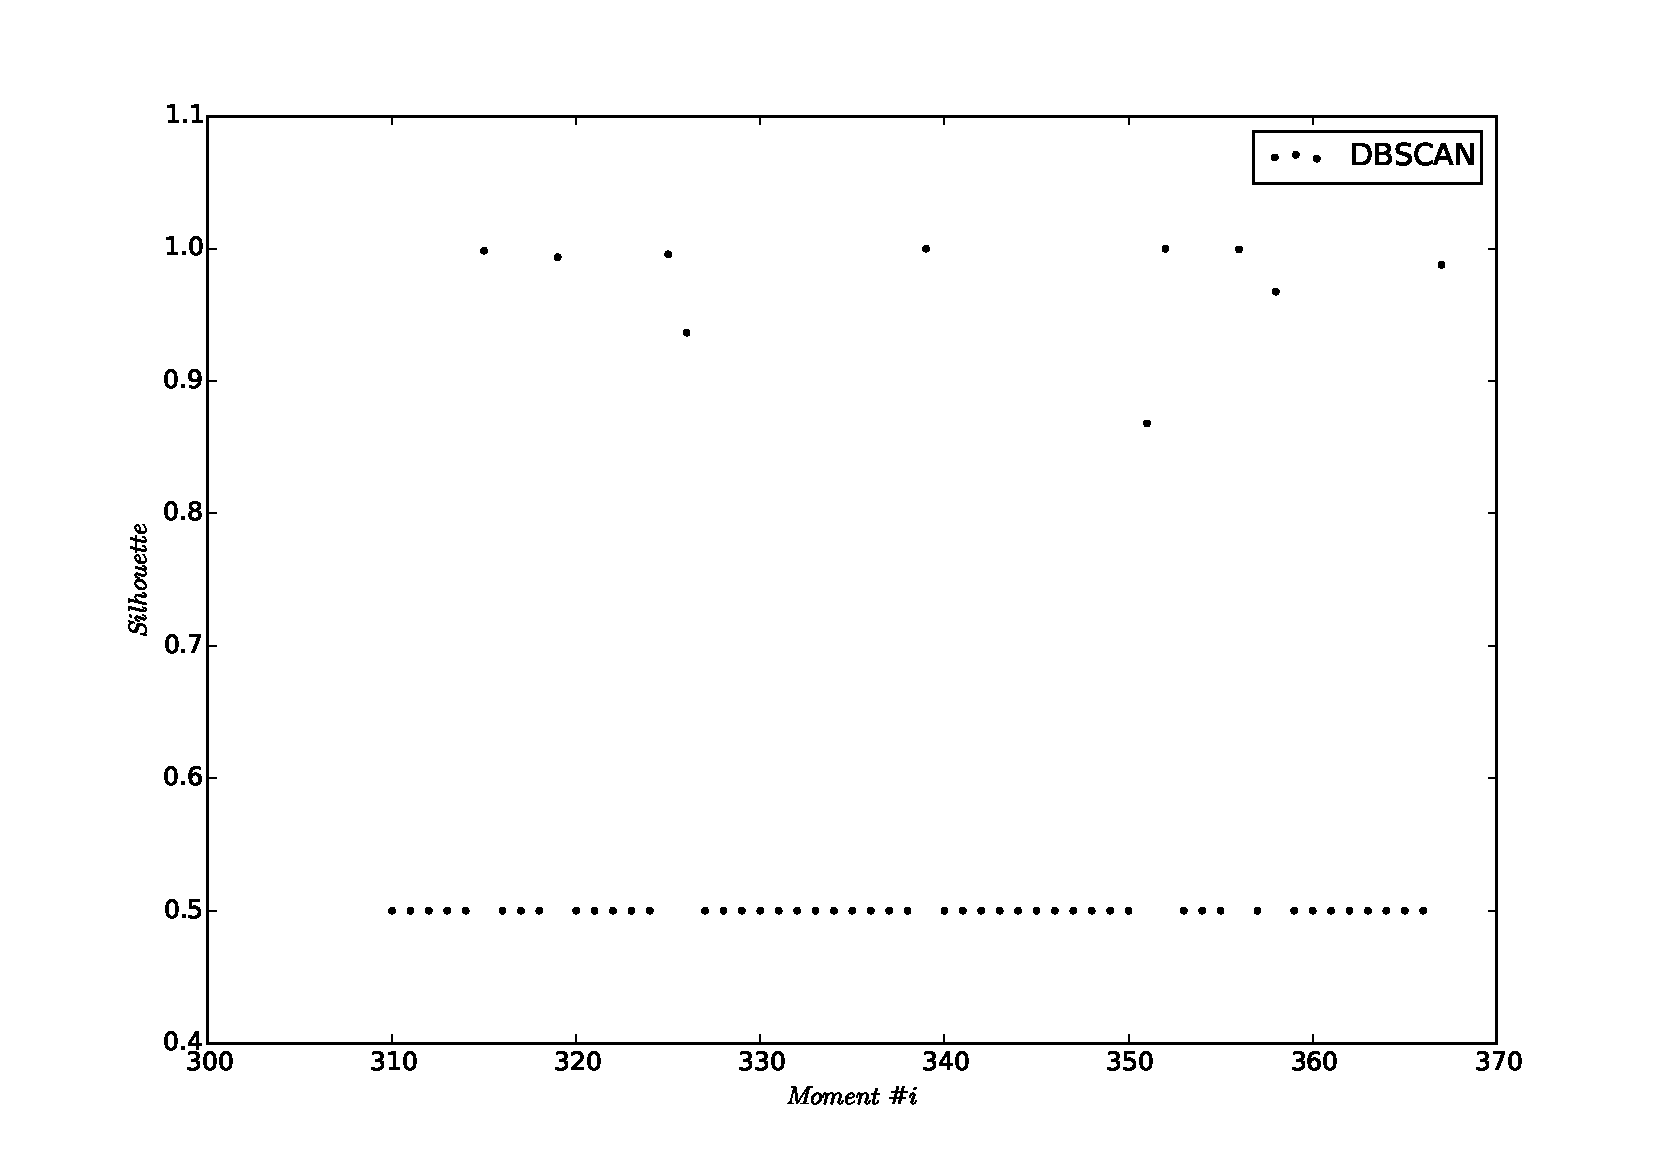
\includegraphics[width=\textwidth]{plots/days_dbscan_silhouette.pdf}
        \caption{Moment-wise silhouette coefficients for DBSCAN for a larger 
        data set. }
        \label{fig:days-dbscan-silhouette}
    \end{subfigure}
    
    \begin{subfigure}[b]{0.45\textwidth}
        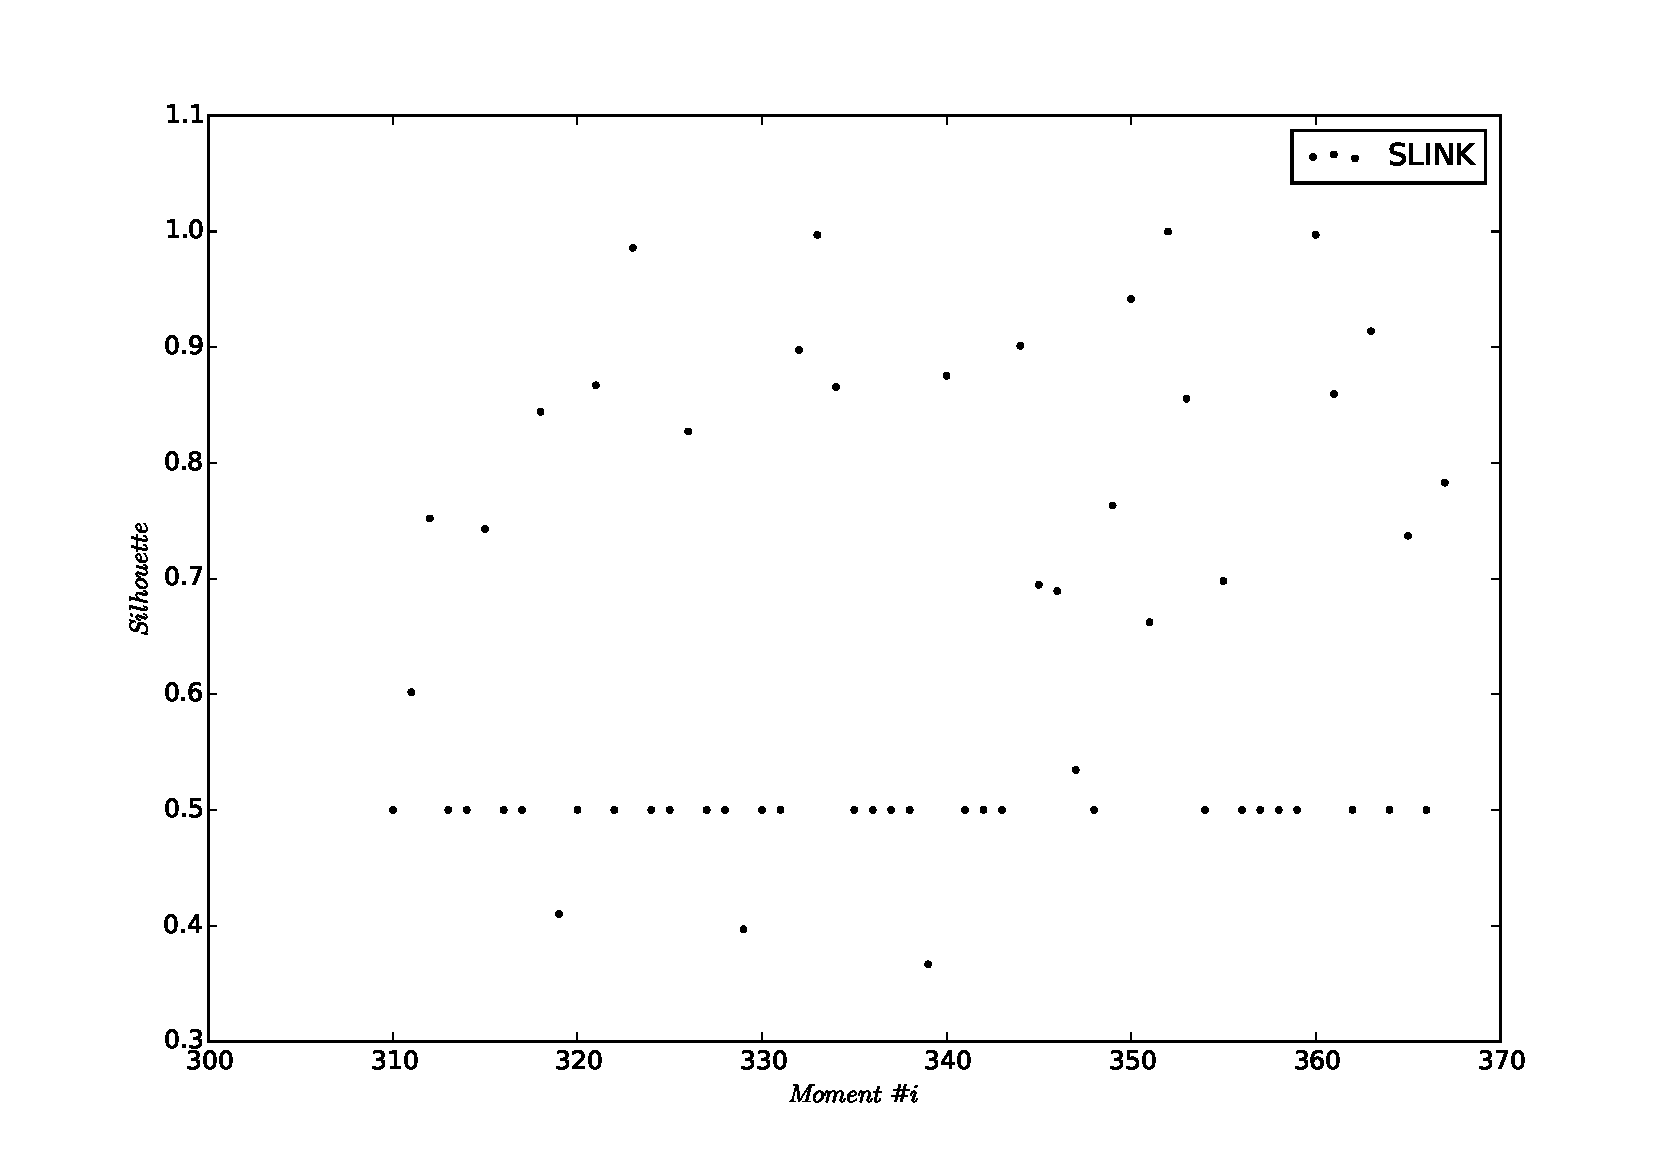
\includegraphics[width=\textwidth]{plots/days_slink_silhouette.pdf}
        \caption{Moment-wise silhouette coefficients for SLINK for a larger 
        data set. }
        \label{fig:days-slink-silhouette}
    \end{subfigure}
\end{figure}

\cleartoleftpage

\subsection{Cluster Detection Comparison}
Different clustering methods result in different clusterings. As an 
attempt to illustrate this, comparisons displaying different clustering
methods and the number of clusters detected in each data set is plotted 
in this section. The regarded data sets are sorted in increasing order 
based on the number of data points in each set.

Although figure~\ref{fig:dbscan-vs-clarans}, \ref{fig:dbscan-vs-slink}
and\ref{fig:clarans-vs-slink} seem somewhat cluttered, the intention here is 
to show the difference in numbers of detected clusters as the data set
increases.

\begin{figure}[ht]
    \centering
    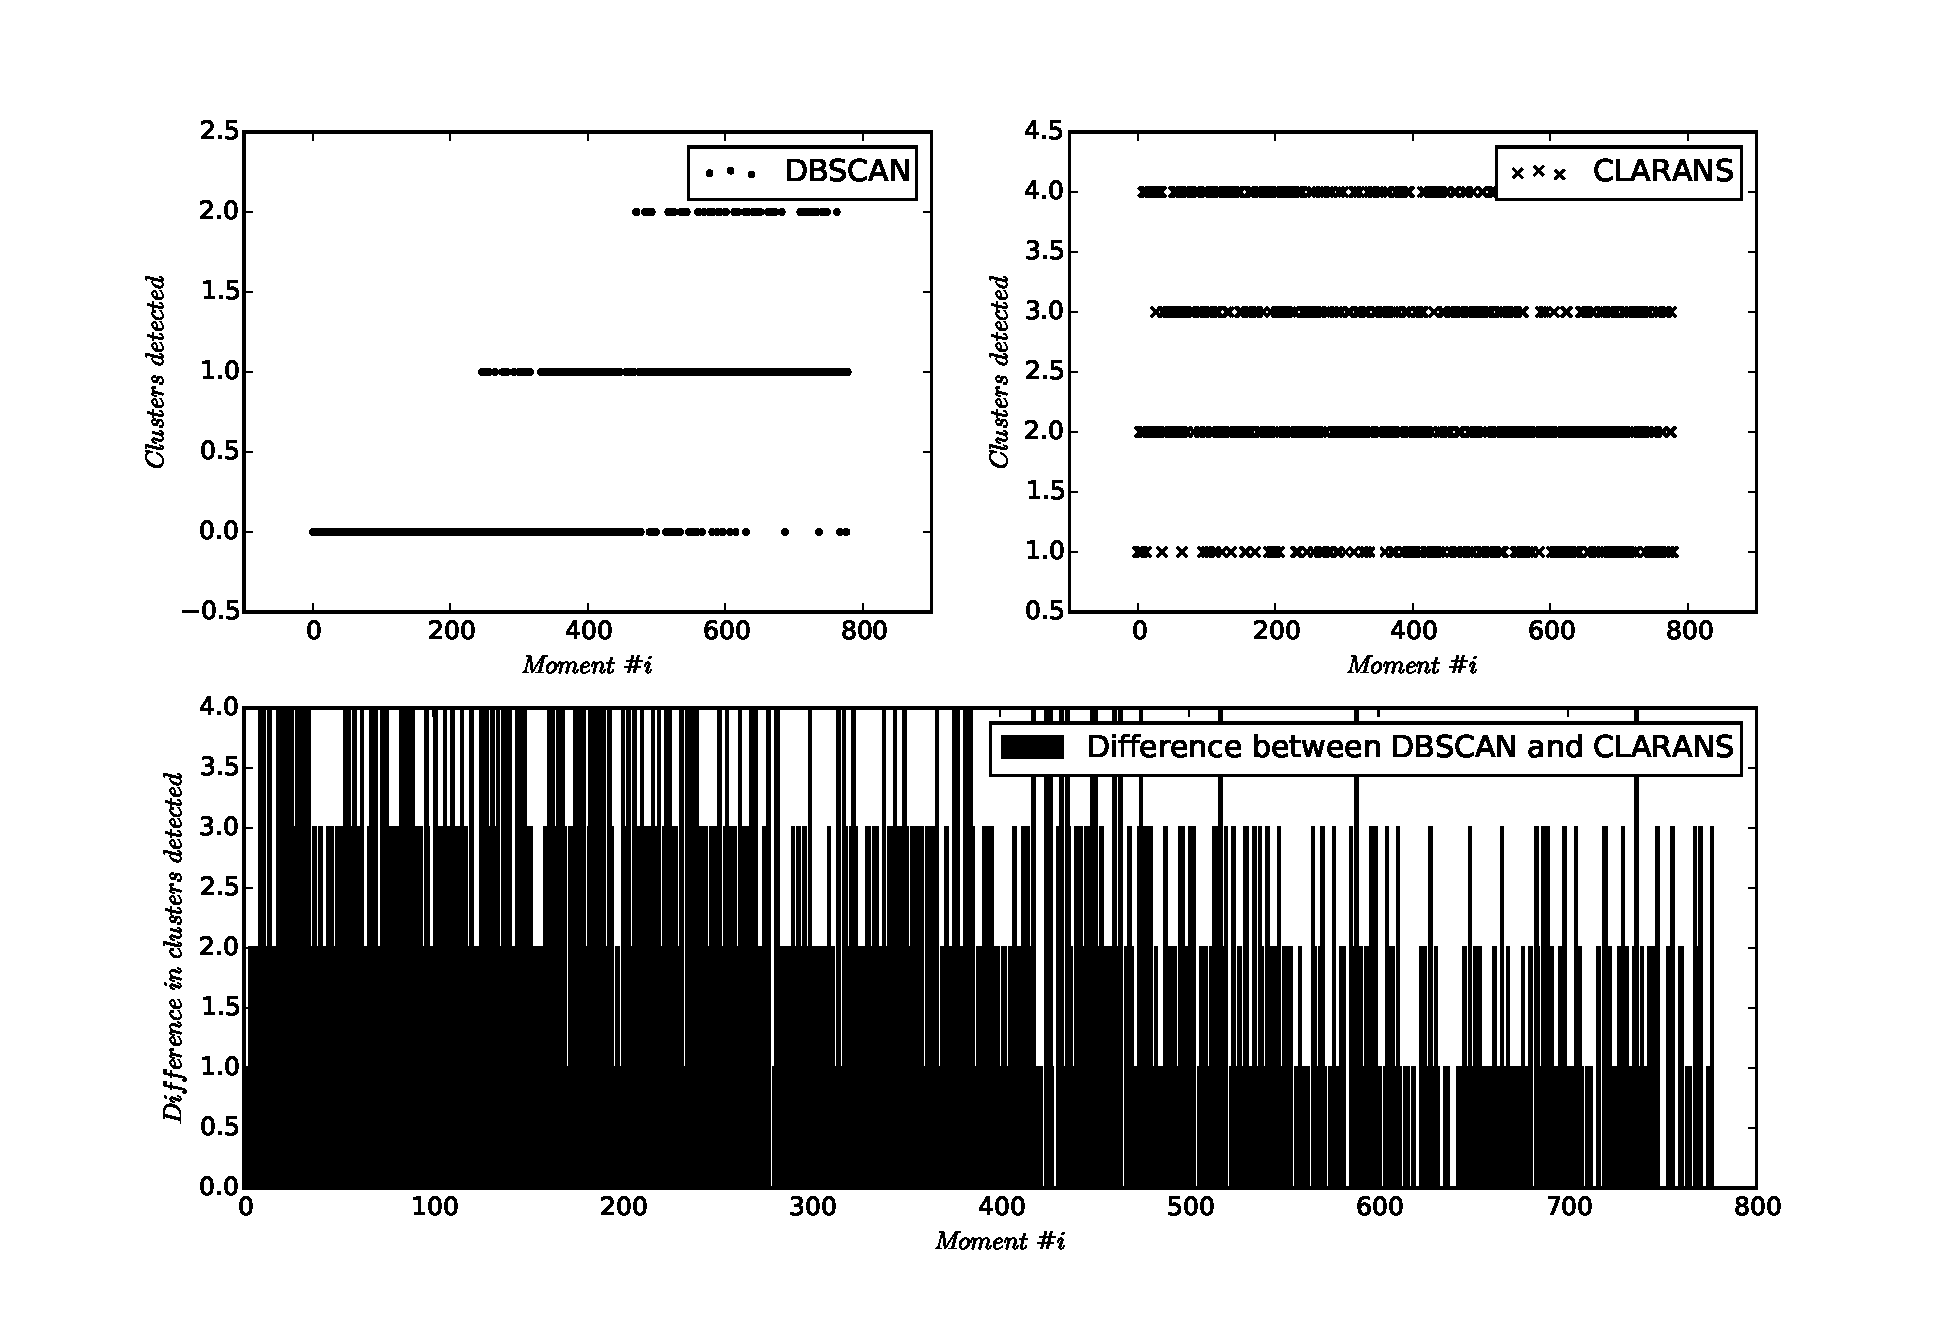
\includegraphics[width=0.9\textwidth]{plots/dbscan_vs_clarans.pdf}
    \caption{Cluster detection, comparison between DBSCAN and CLARANS.
    \label{fig:dbscan-vs-clarans} }
\end{figure}

\begin{figure}[ht]
    \centering
    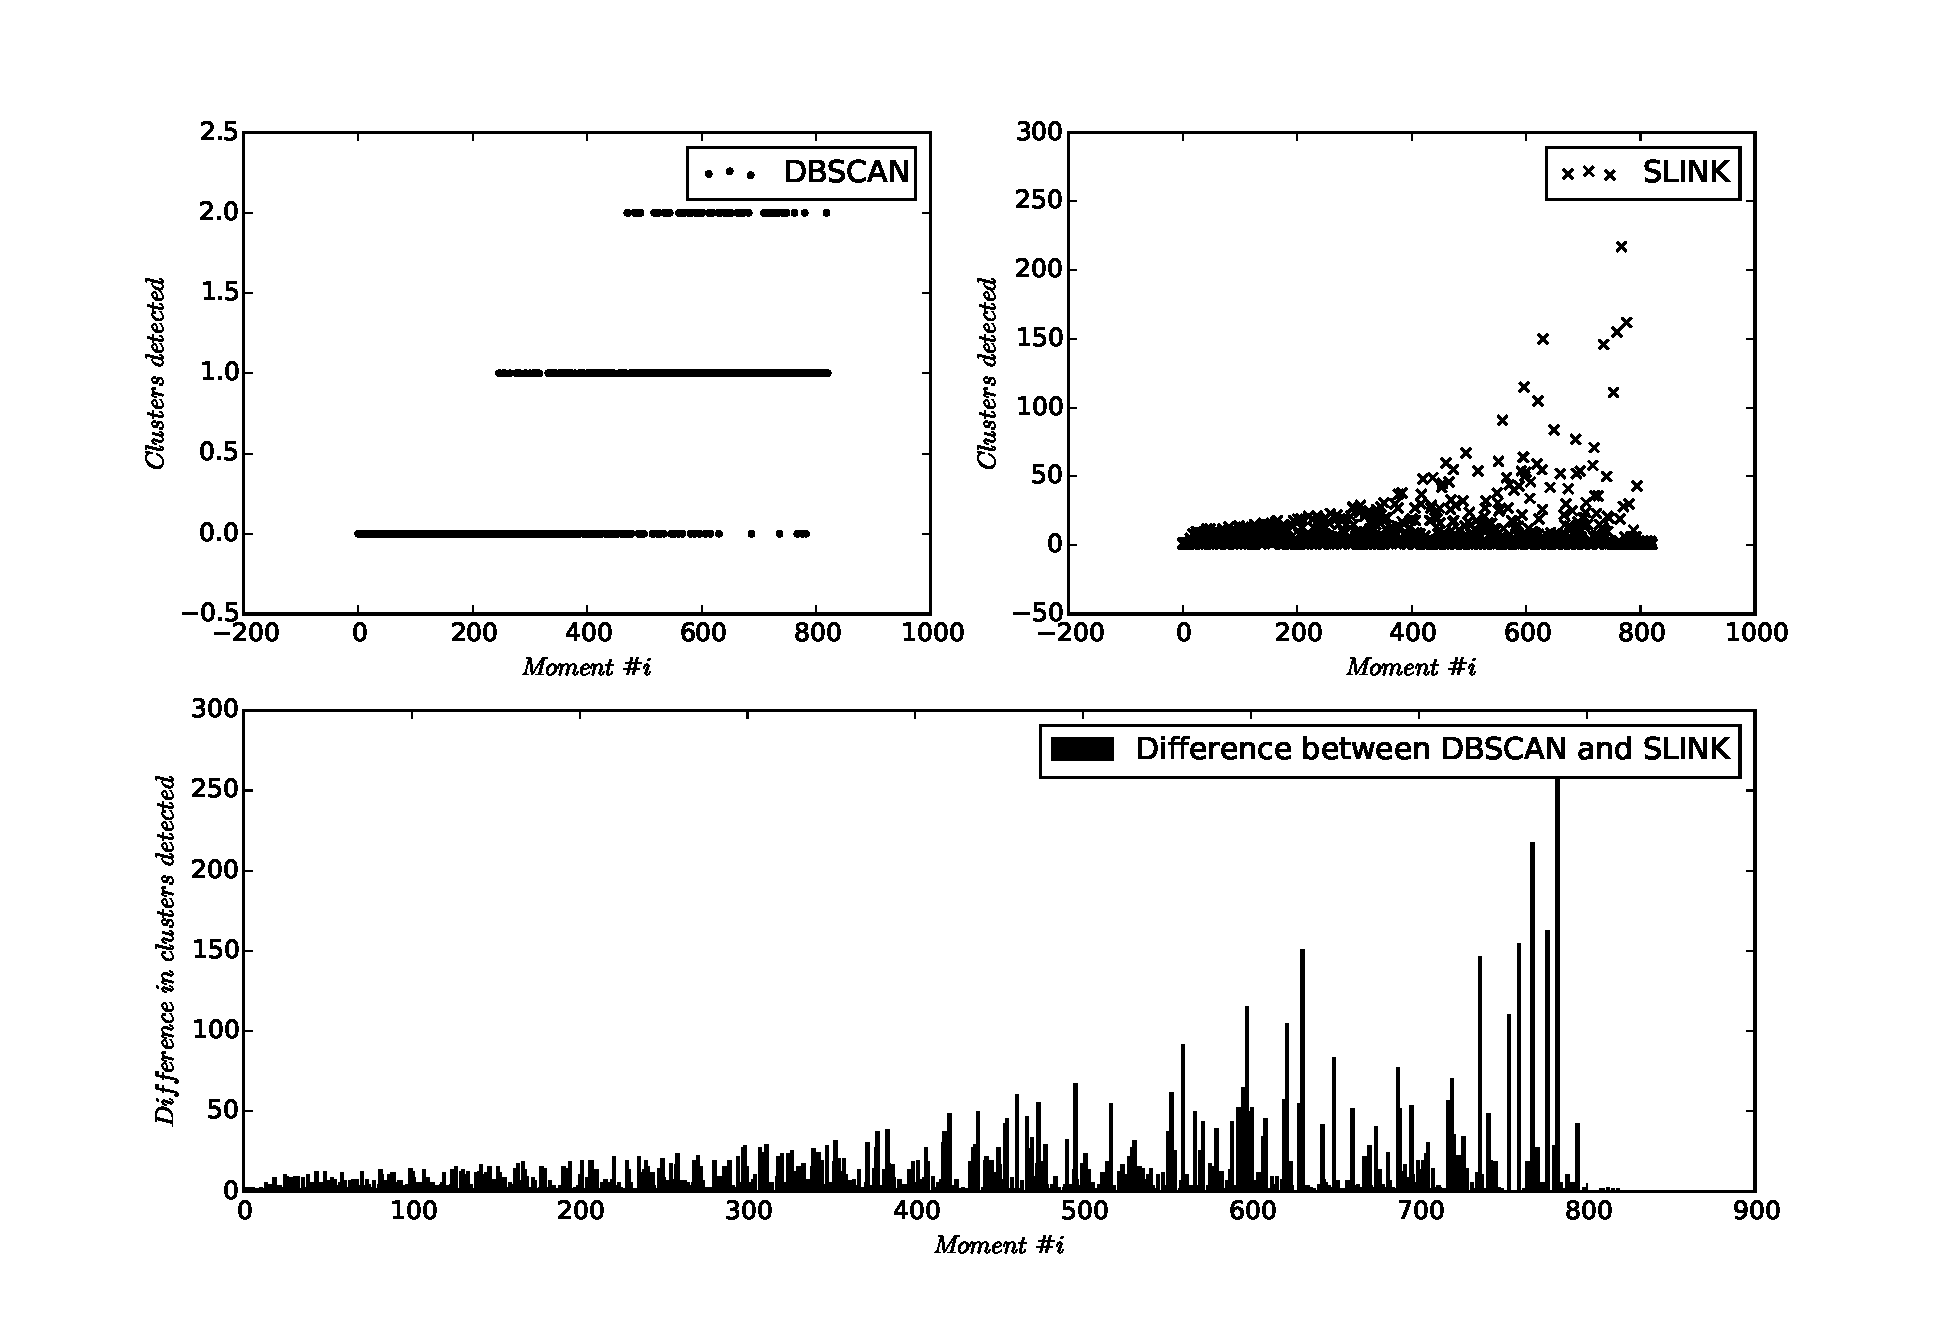
\includegraphics[width=0.9\textwidth]{plots/dbscan_vs_slink.pdf}
    \caption{Cluster detection, comparison between DBSCAN and SLINK.
    \label{fig:dbscan-vs-slink} }
\end{figure}

\begin{figure}[ht]
    \centering
    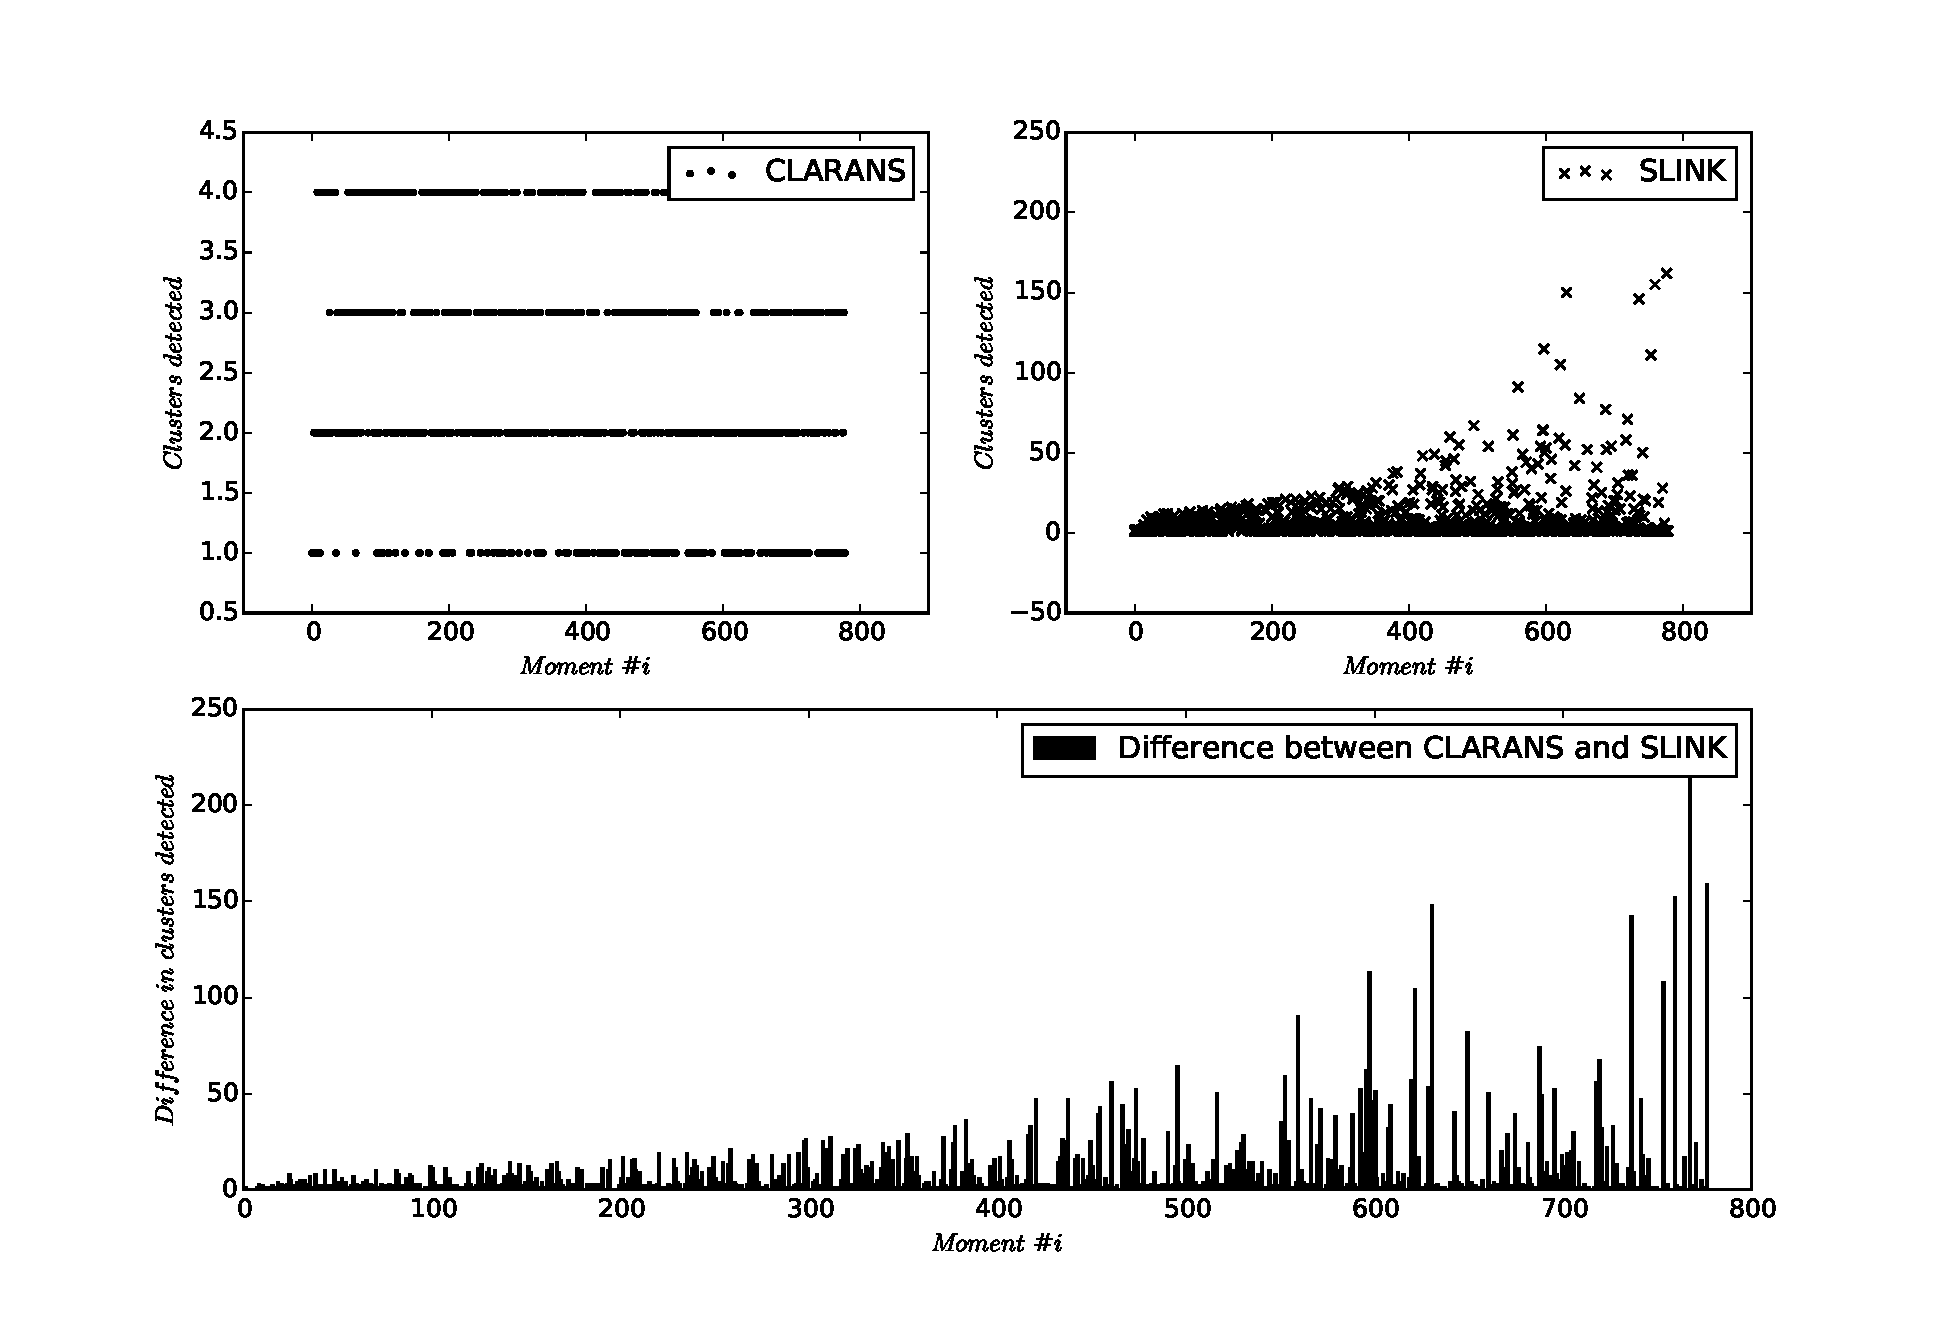
\includegraphics[width=0.9\textwidth]{plots/clarans_vs_slink.pdf}
    \caption{Cluster detection, comparison between CLARANS and SLINK.
    \label{fig:clarans-vs-slink} }
\end{figure}

\cleartoleftpage

\section{Classification}
The classification is conducted after an initial activity detection, in 
this case the above shown spatial clustering. In this stage, the activity
detection is considered correct and which type of clustering algorithm 
that is used is ignored, as all considered and approved algorithms should 
be able to produce desired clusters.

\subsection{Data Set}
The survey based on the user polling in the proof-of-concept implementation
was conducted internally at Narrative.

A total of 11 people participated, and contributed to a total of 62 evaluated
Moment classifications. 

Taking all this into account, it is assumed that the data set still contains 
sufficient and a diverse enough user base to draw conclusions. 

\subsection{Evaluation Overview}

\begin{table}
    \centering
    {\begin{tabular}{ | l | c | l | c | l | c | l | c |}
        \hline
            \multicolumn{2}{|c|}{Movement} &
            \multicolumn{2}{|c|}{Social}   &
            \multicolumn{2}{|c|}{Working}  &
            \multicolumn{2}{|c|}{Indoors} \\
        \hline
            \multicolumn{8}{|c|}{User-assigned values} \\
        \hline
        Stationary  & 40 & Social & 53 & Working    & 57 & Indoors  & 38 \\
        Moving      & 23 & Alone  & 16 & Off Hours  & 12 & Outdoors & 31 \\
        Exercising  &  6 &        &    &            &    &          &    \\
        \hline
            \multicolumn{8}{|c|}{Algorithm-assigned values} \\
        \hline
        Stationary  & 51 & Social & 22 & Working    & 39 & Indoors  & 69 \\
        Moving      & 18 & Alone  & 48 & Off Hours  & 31 & Outdoors & 1 \\
        Exercising  &  1 &        &    &            &    &          &    \\
        \hline
            \multicolumn{8}{|c|}{Correctly assigned according to users.} \\
        \hline
            \multicolumn{2}{|c|}{75.81\%} &
            \multicolumn{2}{|c|}{54.84\%} &
            \multicolumn{2}{|c|}{56.45\%} &
            \multicolumn{2}{|c|}{54.84\%} \\
        \hline
    \end{tabular}}
    \caption{Classification results.} 
    \label{table:classification-values}
\end{table}

\begin{table}
    \centering
    {\begin{tabular}{ | l | c | c |}
        \hline
            Category & False Positive & False Negative \\
        \hline
        Movement    & 1  & 12 \\
        Social      & 0  & 31 \\
        Working     & 27 & 1  \\
        Indoors     & 0  & 31 \\
        \hline
    \end{tabular}}
    \caption{False positives and negatives.} 
    \label{table:false-values-before}
\end{table}

The results after the users responded to the poll is presented in 
table~\ref{table:classification-values}. The quantities 
of assigned classifications by users are shown in the top part of the
table, out of the $69$ assessed Moments. So, for instance, in the 
Movement category there were $40$ Moments assigned as Stationary, 
$23$ as Moving and $6$ as Exercising. In the same manner below that, 
the algorithms assignments to different classes is presented. Note that
this is not the same amount, as these are based on activities, and there
can be (but rarely are) several activities in a Moment.

Table~\ref{table:false-values-before} presents the false negatives and 
positives within each category. The correct assignments are not included
in this table, as only wrong assignments can provide false negatives
and false positives.

\subsection{Second Run}

\begin{table}
    \centering
    {\begin{tabular}{ | l | c | l | c | l | c | l | c |}
        \hline
            \multicolumn{2}{|c|}{Movement} &
            \multicolumn{2}{|c|}{Social}   &
            \multicolumn{2}{|c|}{Working}  &
            \multicolumn{2}{|c|}{Indoors} \\
        \hline
            \multicolumn{8}{|c|}{User-assigned values} \\
        \hline
        Stationary  & 40 & Social & 53 & Working    & 57 & Indoors  & 38 \\
        Moving      & 23 & Alone  & 16 & Off Hours  & 12 & Outdoors & 31 \\
        Exercising  &  6 &        &    &            &    &          &    \\
        \hline
            \multicolumn{8}{|c|}{Algorithm-assigned values} \\
        \hline
        Stationary  & 45 & Social & 27 & Working    & 26 & Indoors  & 44 \\
        Moving      & 18 & Alone  & 43 & Off Hours  & 44 & Outdoors & 26 \\
        Exercising  &  7 &        &    &            &    &          &    \\
        \hline
            \multicolumn{8}{|c|}{Correctly assigned according to users.} \\
        \hline
            \multicolumn{2}{|c|}{78.57\%} &
            \multicolumn{2}{|c|}{62.85\%} &
            \multicolumn{2}{|c|}{73.21\%} &
            \multicolumn{2}{|c|}{71.43\%} \\
        \hline
    \end{tabular}}
    \caption{Classification results after model modification and learning. } 
    \label{table:classification-after-values}
\end{table}

The table~\ref{table:classification-after-values} presents its results in the
same manner as table~\ref{table:classification-values}, but after modification 
of the model via Bayesian learning and lessons learnt after the first user tests. 
The upper area containing the  users assignments remain the same as in 
table~\ref{table:classification-values}, but is kept in this table as well 
for easier reference.

\begin{table}
    \centering
    {\begin{tabular}{ | l | c | c |}
        \hline
            Category & False Positive & False Negative \\
        \hline
        Movement    & 1     & 12 \\
        Social      & 0     & 26 \\
        Working     & 14    & 4  \\
        Indoors     & 7     & 13 \\
        \hline
    \end{tabular}}
    \caption{False positives and negatives after model modification and learning. } 
    \label{table:false-values-after}
\end{table}

In the same way, table~\ref{table:false-values-after} depicts false negatives and 
positives during the run within each category, after the model had been altered.

\clearpage

\subsection{User Grades}

\begin{table}
    \centering
    {\begin{tabular}{ | c | c | c | c | c | c | c | }
        \hline
        Grade & Assigned & Mean &
        \multicolumn{2}{|c|}{False Positive} &
        \multicolumn{2}{|c|}{False Negative} \\
        \hline
        5 & 22 & 0.00 & 0  & 0.00  & 0  & 0.00 \\
        4 & 16 & 1.19 & 4  & 0.25  & 15 & 0.94 \\
        3 & 13 & 2.15 & 8  & 0.62  & 20 & 1.54 \\
        2 & 16 & 2.88 & 14 & 0.88  & 32 & 2.00 \\
        1 & 2  & 3.00 & 2  & 1.00  & 4  & 2.00 \\
        \hline
    \end{tabular}}
    \caption{False positives and negatives correlated
        with user-assigned grades. } 
    \label{table:false-values-vs-grades}
\end{table}

\begin{table}
    \centering
    {\begin{tabular}{ | l | c | c | c | c | c | c | }
        \hline
        User & Count & Mean Grade\\
        \hline
        User \#1 & 17 & 4.47 \\
        User \#2 & 7  & 3.14 \\
        User \#3 & 12 & 3.33 \\
        User \#4 & 8  & 3.5  \\
        User \#5 & 7  & 4.0  \\
        User \#6 & 8  & 2.63 \\
        \hline
    \end{tabular}}
    \caption{Mean grades and number of classifications distributed 
        among the users with most responses.} 
    \label{table:user-wise-mean-grade}
\end{table}

\emph{
    The reason that the number of values in the Assigned column
    of table~\ref{table:false-values-vs-grades} does not sum to
    62 as the number of examined Moments were, is simply that these
    are scores for each activity, not for each Moment assessed, as 
    there can be several activities in a Moment. }

Table~\ref{table:false-values-vs-grades} shows the correlation 
between false positives and negatives, along with the grades 
that users have assigned to the classification. 
The column marked mean shows the mean number of errors in order a
classification getting the corresponding user grade. The first value 
in the false-columns shows the total number of false positives 
and negatives respectively in classifications that have received 
a certain grade. The real-valued column shows the number of false 
positives respectively per classification in that category. 
